\documentclass[9pt]{beamer}
\mode<presentation>

% Theme choice:
\usetheme{Madrid}%Darmstadt

\usecolortheme[RGB={0,100,50}]{structure}
 \usefonttheme{structurebold}
\setbeamercovered{invisible}
%\setbeamertemplate{navigation symbols}{}
\usepackage{dynblocks}
\usepackage{textpos}
\usepackage{amsfonts}
\usepackage{amsmath}
\usepackage{amssymb}
\usepackage{amsthm}
\usepackage{mathtools}
\usepackage{dutchcal}
\usepackage{hyperref}
\usepackage[utf8]{inputenc}
\usepackage[T1]{fontenc}
\usepackage[french]{babel}
\usepackage{enumitem}
\usepackage{array}
\usepackage{tabularx}
\usepackage{booktabs}

\usepackage[affil-it]{authblk}
\usepackage{toolbox}
\usepackage{lmodern}

% Chemins des images : logo et captures dans ../images/, diagrammes UML
% dans ../diagrammes/
\graphicspath{{../images/}{../diagrammes/}}

% ── Harmonisation des couleurs ────────────────────────────────────────
% Le vert du thème est défini une seule fois et sert partout : puces,
% accents, filets. Les diagrammes PlantUML emploient le même #006432.
\definecolor{vertPlainte}{RGB}{0,100,50}
\definecolor{vertClair}{RGB}{228,240,233}

% Toutes les listes prennent ce vert : plus aucune puce en vert vif.
\setlist[itemize,1]{label=$\bullet$, font=\LARGE\color{vertPlainte}, itemsep=2pt}
\setlist[itemize,2]{label=$\circ$, font=\normalsize\color{vertPlainte}, itemsep=1pt}

% Ligne de synthèse placée sous une figure.
\newcommand{\aretenir}[1]{%
  \vspace{2pt}%
  \begin{center}\small\color{vertPlainte}\textbf{#1}\end{center}}

\makeatletter
\patchcmd{\@maketitle}{\LARGE \@title}{\fontsize{14}{19.2}\selectfont\@title}{}{}
\makeatother

\renewcommand\Authfont{\fontsize{14}{14.4}\selectfont}
\renewcommand\Affilfont{\fontsize{14}{10.8}\itshape}

% Title page details:
\title[Master Professionnel SIGL]{CONCEPTION ET RÉALISATION D'UNE PLATEFORME DE DÉPÔT ET DE TRAITEMENT NUMÉRIQUE DES PLAINTES CITOYENNES}

\institute[Access Finance \& RH --- UY1]{\textbf{\large
Présenté par :\\
TCHOUALA NODEM BOREL\\[0.8em]
Supervisé par :\\
Dr. NZEKON NZEKO'O ARMEL JACQUES\\
M. NDJON MBOG THIERRY}
 \begin{center}
  
\includegraphics[width=0.15\textwidth]{Logo.png}

\end{center}
}
\date{Année académique 2025--2026}

\usepackage[pscoord]{eso-pic}


\begin{document}

\frame[plain]{\titlepage}

\begin{frame}{PLAN DE TRAVAIL}
  \tableofcontents
\end{frame}

%####################################################

\section{INTRODUCTION}

\begin{frame}{Contexte et problématique}
    \begin{center}
    \begin{figure}[htp]
  
\includegraphics[width=0.42\textwidth]{problematique_flux.png}
  \label{fig:intro}
\end{figure}
\end{center}
    \begin{block}{}
   Comment concevoir une plateforme permettant à un citoyen de déposer une plainte de manière guidée, à un commissariat de coter et d'instruire l'enquête, et à la procédure d'être suivie et tracée, tout en mobilisant l'intelligence artificielle pour alléger la rédaction des procès-verbaux sans dessaisir l'officier de police judiciaire de sa responsabilité ?
\end{block}
\end{frame}

\begin{frame}{Le dépôt de plainte est un acte juridique}
  \begin{itemize}
    \item Le dépôt de plainte engage le commissariat dès sa réception;
    \item Il est encadré par le Code de procédure pénale;
    \item Le procès-verbal est un acte de l'officier de police judiciaire;
    \item Le dématérialiser ne peut donc pas se réduire à un formulaire en ligne;
    \item Enjeu : préserver la valeur probante tout en supprimant les frictions.
  \end{itemize}
\end{frame}

%####################################################

\section{STRUCTURE DE STAGE}

\begin{frame}{Access Finance \& RH SARL et missions confiées}
  \begin{columns}
    \begin{column}{0.52\textwidth}
      \begin{block}{L'entreprise}
      \begin{itemize}
        \item Solutions numériques sur mesure;
        \item Clients publics et privés;
        \item Circuits de décision courts;
        \item Stage de six mois en équipe de développement.
      \end{itemize}
      \end{block}
      \begin{block}{Missions}
      \begin{itemize}
        \item Auditer la procédure existante;
        \item Concevoir l'architecture de la solution;
        \item Développer la plateforme en full-stack;
        \item Intégrer l'intelligence artificielle générative;
        \item Conduire la recette et documenter.
      \end{itemize}
      \end{block}
    \end{column}
    \begin{column}{0.44\textwidth}
      \begin{figure}
        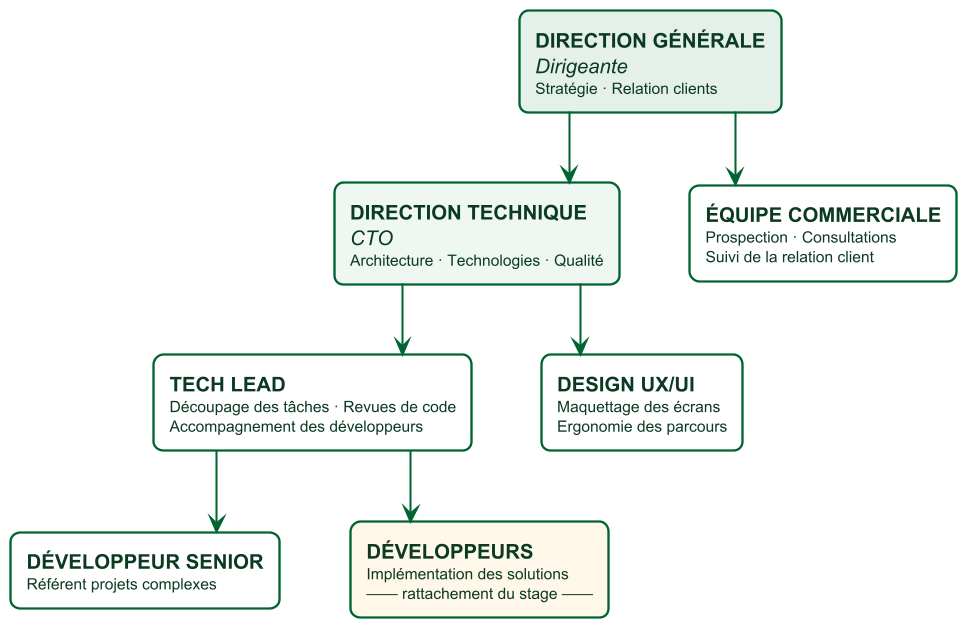
\includegraphics[width=0.98\textwidth]{organigramme_klivar.png}
        \label{fig:orga}
      \end{figure}
    \end{column}
  \end{columns}
\end{frame}

%####################################################

\section{ETUDE DE L'EXISTANT}

\begin{frame}[c]{La procédure actuelle, entièrement manuelle}
\small Audit de deux commissariats de Yaoundé, Ngoa-Ekélé et Mimboman : entretiens semi-directifs anonymisés et observation directe du flux de travail.
\vspace{4pt}
\begin{figure}[htp]
 \centering
  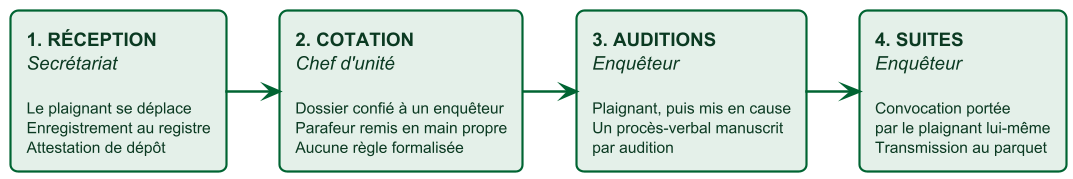
\includegraphics[width=\linewidth]{procedure_actuelle.png}
  \label{fig:proc_actuelle}
\end{figure}
\aretenir{Aucune trace numérique : ni le délai de cotation ni celui du traitement ne sont mesurables.}
\end{frame}

\begin{frame}{Le constat qui a orienté toute la conception}
  \begin{itemize}
    \item C'est \textbf{en principe le plaignant lui-même} qui remet la convocation au mis en cause;
    \item Un policier ne l'assiste que s'il redoute des représailles;
    \item Or l'auteur présumé est souvent un proche ou un voisin;
    \item Cette exposition peut dissuader de poursuivre la procédure;
    \item Voire de la déclencher.
  \end{itemize}
\end{frame}

\begin{frame}{Difficultés relevées}
\small
\begin{tabularx}{\textwidth}{@{}c>{\raggedright\arraybackslash}X>{\raggedright\arraybackslash}X@{}}
  \toprule
  \textbf{\#} & \textbf{Difficulté} & \textbf{Impact} \\
  \midrule
  1 & Le plaignant ne sait ni lire ni écrire & Dépendance à un tiers, confidentialité fragilisée \\
  \addlinespace
  2 & Il peine à exposer les faits clairement & Dossier incomplet, PV lacunaire \\
  \addlinespace
  3 & Le mis en cause refuse de signer le PV & Contentieux, risque de vice de forme \\
  \addlinespace
  4 & Rédaction manuscrite longue et répétitive & Temps soustrait à l'enquête \\
  \bottomrule
\end{tabularx}
\aretenir{Trois difficultés sur quatre portent sur la qualité de la déclaration.}
\end{frame}

\begin{frame}{Ce qui existe ailleurs, et pourquoi développer}
\small
\begin{tabularx}{\textwidth}{@{}l>{\raggedright\arraybackslash}X>{\raggedright\arraybackslash}X@{}}
  \toprule
  \textbf{Dispositif} & \textbf{Couvre} & \textbf{Ne couvre pas} \\
  \midrule
  \textbf{France} \newline Visioplainte, 2024
    & Dépôt à distance, visioconférence, PV signé sans déplacement
    & Réservé aux atteintes aux biens dont l'auteur est inconnu \\
  \addlinespace
  \textbf{Sénégal} \newline PSIC, 2026
    & Signalement des cyberinfractions
    & Périmètre thématique, rien en aval du signalement \\
  \addlinespace
  \textbf{Cameroun} \newline DGSN / GIZ, 2022
    & Plaintes des usagers contre la police
    & Objet distinct : contrôle interne, pas le dépôt pénal \\
  \bottomrule
\end{tabularx}
\vspace{4pt}
\small Tous s'arrêtent au dépôt : ni cotation, ni auditions, ni procès-verbaux. Aucun ne traite nos constats.
\aretenir{D'où le choix de développer, en gardant le dispositif français comme piste d'évolution.}
\end{frame}

%####################################################

\section{MISE EN PLACE DE LA SOLUTION}

\begin{frame}{Objectifs et démarche}
  \begin{columns}
    \begin{column}{0.5\textwidth}
      \begin{block}{Objectifs}
      \begin{itemize}
        \item Supprimer le déplacement obligatoire;
        \item Rattacher le dossier au commissariat compétent;
        \item Réduire la charge de rédaction des PV;
        \item Permettre au plaignant de suivre son dossier;
        \item Garantir la traçabilité;
        \item Couvrir quatre profils d'utilisateurs.
      \end{itemize}
      \end{block}
    \end{column}
    \begin{column}{0.47\textwidth}
      \begin{block}{Agile Scrum, six sprints}
      \scriptsize
      \begin{tabularx}{\textwidth}{@{}l>{\raggedright\arraybackslash}X@{}}
        \toprule
        \textbf{\#} & \textbf{Livré} \\
        \midrule
        1 & Authentification, profils, navigation par rôle \\
        2 & Dépôt en cinq étapes, cascade géographique \\
        3 & Questions complémentaires, dictée, rédaction assistée \\
        4 & Espace enquêteur, procès-verbaux, convocations \\
        5 & Espace commissaire, cotation, statistiques \\
        6 & Journal d'audit, pièces PDF, recette \\
        \bottomrule
      \end{tabularx}
      \end{block}
    \end{column}
  \end{columns}
\end{frame}

\begin{frame}[c]{Architecture fonctionnelle : ce que fait la plateforme}
\begin{figure}[htp]
 \centering
  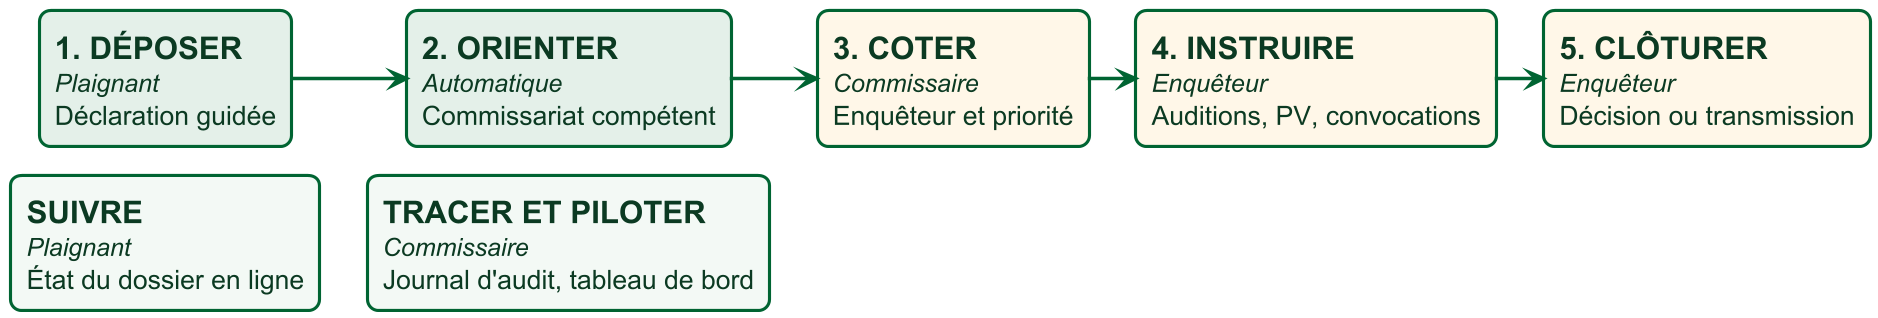
\includegraphics[width=\linewidth]{architecture_fonctionnelle.png}
  \label{fig:archi_fonc}
\end{figure}
\aretenir{Cinq temps, un acteur responsable par temps, et deux fonctions qui traversent tout le cycle.}
\end{frame}

\begin{frame}{Architecture de conception : les modules}
\begin{figure}[htp]
 \centering
  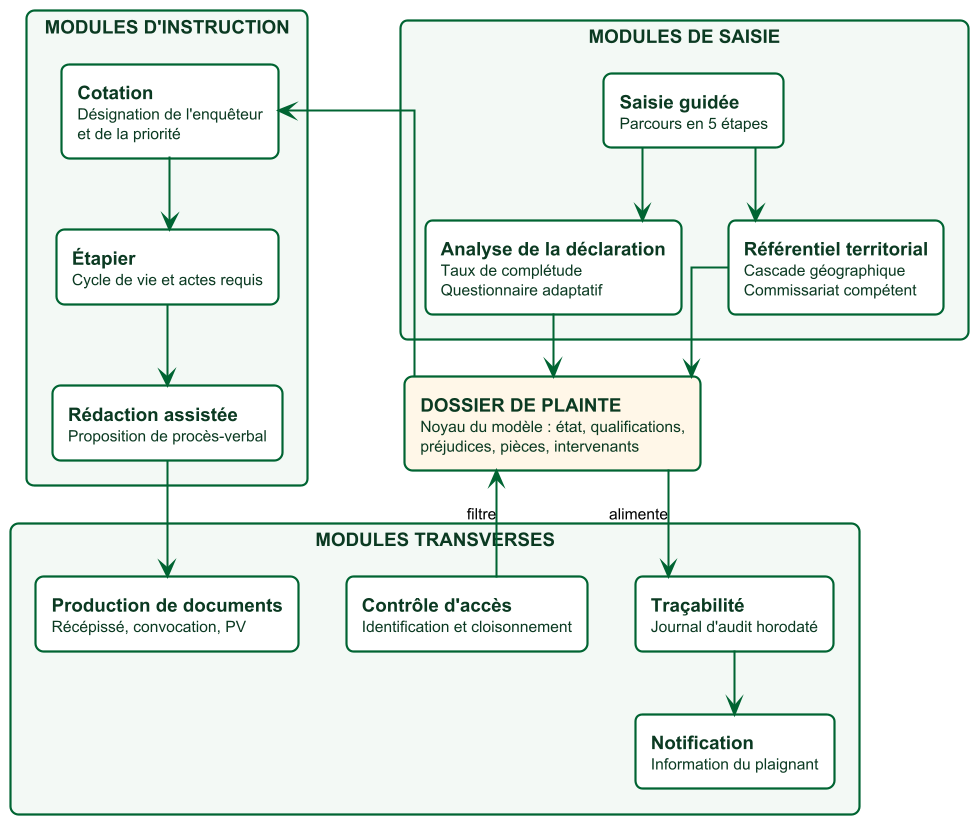
\includegraphics[height=0.74\textheight,keepaspectratio]{architecture_conception.png}
  \label{fig:archi_conc}
\end{figure}
\aretenir{Tout converge vers le dossier de plainte : aucun groupe de modules n'en dépend d'un autre.}
\end{frame}

\begin{frame}{Architecture d'implémentation : les technologies}
\begin{figure}[htp]
 \centering
  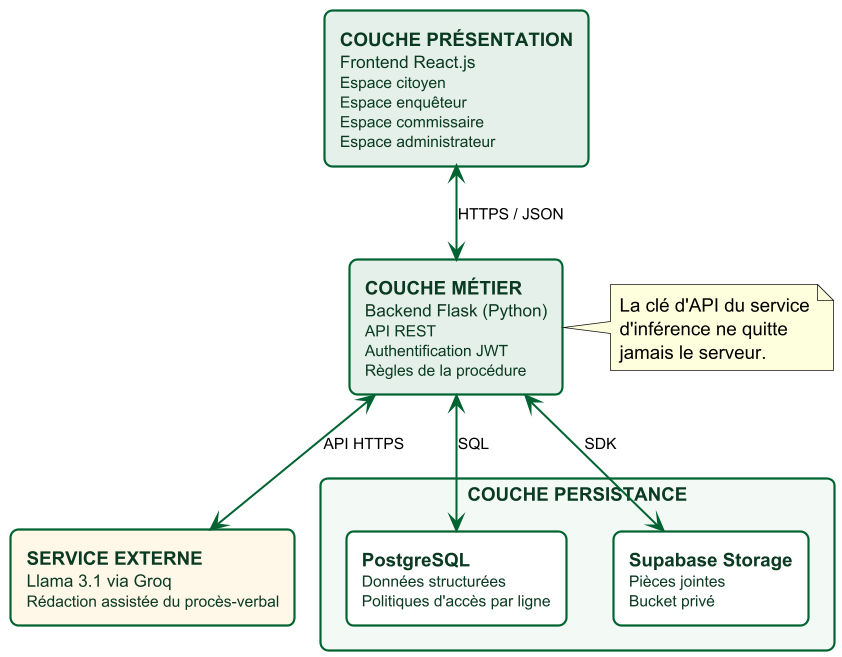
\includegraphics[height=0.74\textheight,keepaspectratio]{architecture.png}
  \label{fig:archi_impl}
\end{figure}
\aretenir{Trois tiers découplés, et un appel d'inférence qui ne part jamais du navigateur.}
\end{frame}

\begin{frame}[c]{Le dépôt guidé, en cinq étapes}
\begin{figure}[htp]
 \centering
  
\includegraphics[width=\linewidth]{crop_depot_etapes.png}
  \label{fig:ecran_depot}
\end{figure}
\vspace{2pt}
  \begin{itemize}
    \item Nature de l'infraction et cascade Région, Département, Arrondissement, Quartier;
    \item Déclaration des faits, avec dictée vocale optionnelle;
    \item Identité du mis en cause, facultative si elle est inconnue;
    \item Questions complémentaires propres à la nature déclarée;
    \item Aperçu, signature et délivrance d'un récépissé PDF.
  \end{itemize}
\aretenir{Le commissariat compétent s'affiche avant même le dépôt.}
\end{frame}

\begin{frame}{Deux pourcentages qu'il ne faut pas confondre}
  \begin{columns}[t]
    \begin{column}{0.48\textwidth}
      \begin{block}{Complétude de la déclaration}
      \begin{itemize}
        \item S'adresse au \textbf{citoyen};
        \item Mesure la richesse du récit : objet, moment, suspect, témoins, justificatif;
        \item Les éléments manquants deviennent les questions de l'étape 4.
      \end{itemize}
      \end{block}
    \end{column}
    \begin{column}{0.48\textwidth}
      \begin{block}{Avancement du dossier}
      \begin{itemize}
        \item S'adresse au \textbf{commissariat};
        \item Mesure la procédure accomplie : étapes franchies et actes réalisés;
        \item Ne se saisit jamais à la main.
      \end{itemize}
      \end{block}
    \end{column}
  \end{columns}
\aretenir{Les confondre ferait paraître avancé un dossier simplement bien raconté.}
\end{frame}

\begin{frame}{Rédaction assistée du procès-verbal}
  \begin{itemize}
    \item Projet de PV au format du template institutionnel, en-tête compris;
    \item Appel exclusivement côté serveur : la clé d'API ne quitte jamais le backend;
    \item Chaque correction de l'enquêteur est horodatée et conservée.
  \end{itemize}
\vspace{2pt}
\begin{figure}[htp]
 \centering
  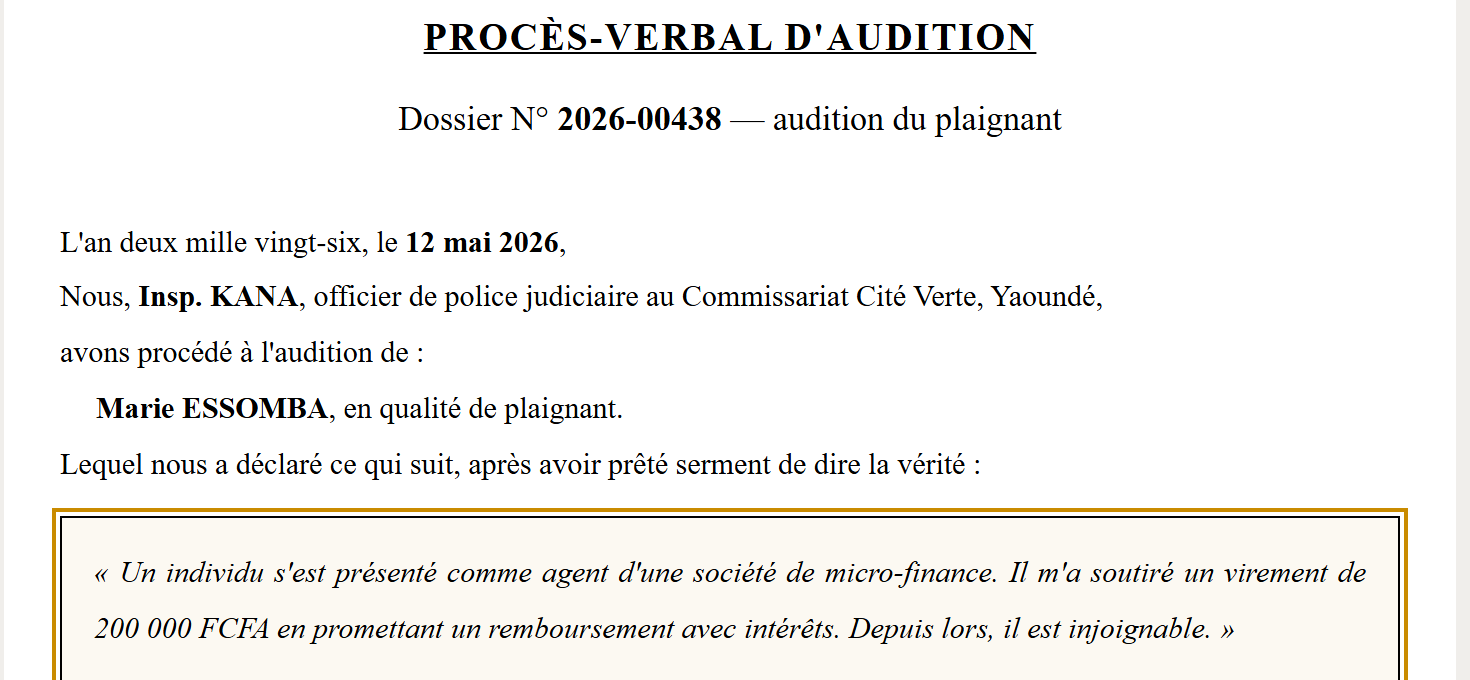
\includegraphics[width=0.95\linewidth]{crop_pv.png}
  \label{fig:ecran_pv}
\end{figure}
\aretenir{Une proposition, jamais un acte : l'IA ne se substitue pas à l'officier de police judiciaire.}
\end{frame}

\begin{frame}{Coter et piloter : l'espace du commissaire}
  \begin{itemize}
    \item Cotation à un enquêteur avec priorité, la charge de chacun étant visible avant de coter;
    \item Journal d'audit horodaté, et cloisonnement doublé au niveau du SGBD.
  \end{itemize}
\vspace{2pt}
\begin{figure}[htp]
 \centering
  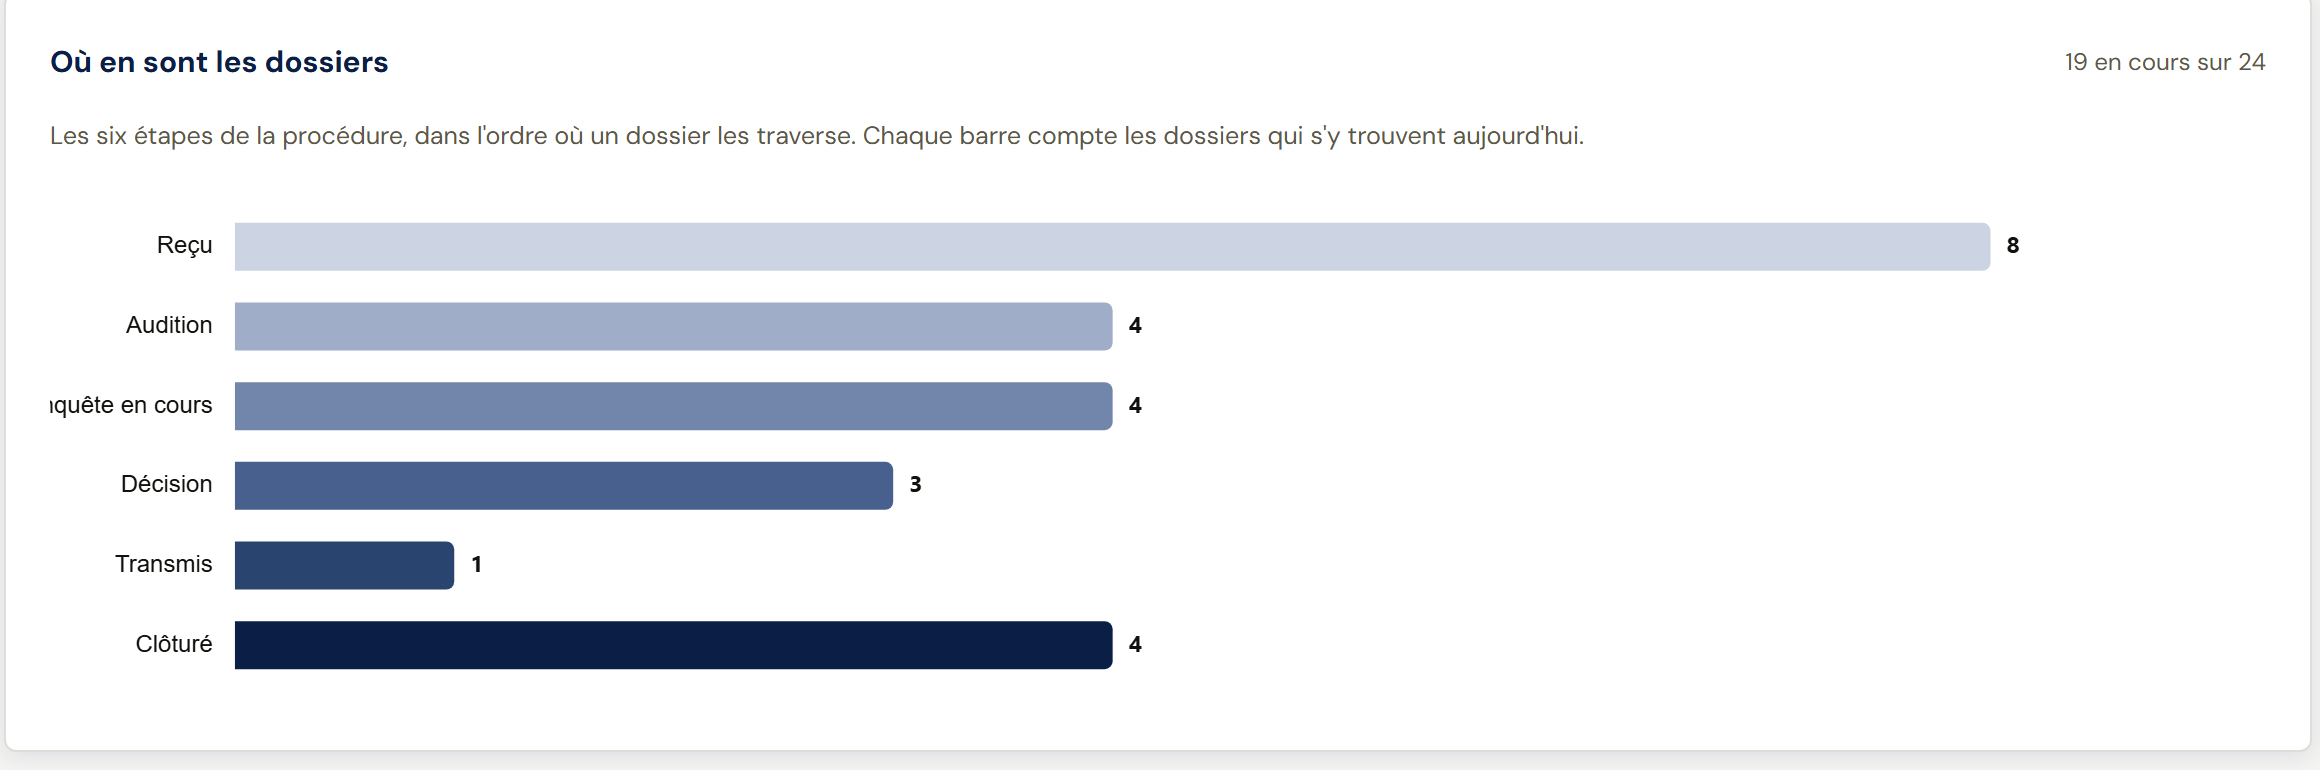
\includegraphics[width=\linewidth]{crop_dashboard_etapes.png}
  \label{fig:dashboard}
\end{figure}
\aretenir{Ce que la procédure manuelle ne permettait pas : savoir où en sont les dossiers.}
\end{frame}

%####################################################

\section{OUTILS ET LOGICIELS}

\begin{frame}{OUTILS ET LOGICIELS}
\begin{columns}
    \begin{column}{0.45\textwidth}
        \begin{block}{Technologies}
            \begin{itemize}
                \item React.js 
\includegraphics[width=0.08\textwidth]{react.png}
                \item Flask (Python)
                \item PostgreSQL
                \item Supabase Storage
                \item Llama 3.1 via Groq 
\includegraphics[width=0.08\textwidth]{grok_ai.png}
            \end{itemize}
        \end{block}

        \begin{block}{Environnement logiciel}
            \begin{itemize}
                \item Visual Studio Code
                \item Git et GitHub
                \item Docker
                \item Postman
            \end{itemize}
        \end{block}
    \end{column}

    \begin{column}{0.45\textwidth}
        \begin{block}{Ce qui a tranché}
            \begin{itemize}
                \item \textbf{Flask} :  Offre un cadre léger, flexible et rapide pour développer des applications web ou des API en Python. Il s'intègre facilement aux services d'API tels que l'API de Grok.;
                \item \textbf{Groq} : gratuit et très rapide;
                \item \textbf{PostgreSQL} : les \emph{données} --- comptes, dossiers, historique;
                \item \textbf{Supabase Storage} : les \emph{fichiers} --- pièces jointes, procès-verbaux, convocations.
            \end{itemize}
        \end{block}
    \end{column}
\end{columns}
\end{frame}

%####################################################

\section{RESULTATS}

\begin{frame}[c]{Démonstration}
\begin{figure}[htp]
 \centering
  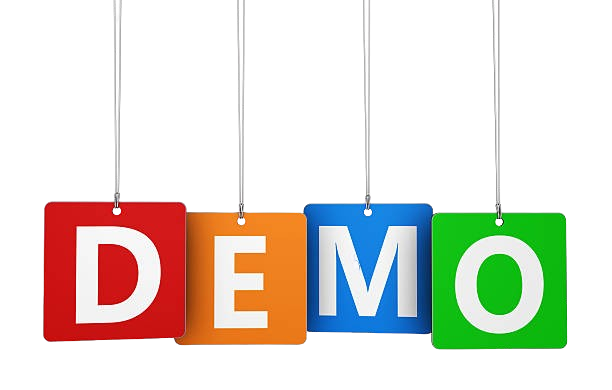
\includegraphics[width=0.42\textwidth]{demo_icon.png}
  \label{fig:demo}
\end{figure}
\end{frame}

\begin{frame}{Ce que le mémoire ne prétend pas}
  \begin{itemize}
    \item Aucun chiffre sur la durée de cotation ou de traitement : ces durées relèvent du commissariat et l'absence de traçabilité les rendait inconnaissables;
    \item Les mesures viennent de la recette, non de l'exploitation réelle;
    \item Le refus de signature du PV n'est pas résolu : la plateforme en garde la trace, elle ne l'empêche pas;
    \item La transcription vocale reste imparfaite sur les noms propres et les toponymes;
    \item Aucun test de charge n'a été mené.
  \end{itemize}
\end{frame}

%####################################################

\section{CONCLUSION}

\begin{frame}{CONCLUSION}

\begin{itemize}

    \item \textbf{Objectif : }
    \begin{itemize}
    \item Dématérialiser le dépôt et le traitement des plaintes citoyennes, jusqu'alors entièrement manuels.
    \end{itemize}
    \item \textbf{Solution : }
        \begin{itemize}
  \item Dépôt guidé en ligne, sans déplacement;
  \item Rattachement automatique au commissariat compétent;
  \item Cotation, instruction et convocations outillées;
  \item Procès-verbal assisté, validé par l'officier de police judiciaire;
  \item Traçabilité horodatée de toutes les transitions.
  \end{itemize}
  \item \textbf{Limites : }
     \begin{itemize}
  \item Transcription vocale imparfaite, relecture obligatoire;
  \item Mesures issues de la recette, non de l'exploitation réelle.
  \end{itemize}
\item \textbf{Perspectives : }
    \begin{itemize}
  \item Instrumenter la plateforme puis déployer sur un commissariat pilote;
  \item Transcription vocale côté serveur, ouvrant aux langues nationales;
  \item Transmission dématérialisée des dossiers au parquet.
\end{itemize}
     \end{itemize}

\end{frame}

\begin{frame}{}
   \centering \Large MERCI POUR VOTRE ATTENTION
\end{frame}

\end{document}
